%!TEX root = 00_main.tex

\section{Experiments}

We evaluated the usefulness of our synthetic data generation method on two sample problems, eye registration and gaze estimation.

\commentA{briefly say something about significance/importance of both problems, more in corresponding subsections}

\subsection{Eye-Region Registration}

\commentA{results look pretty good already, I suggest put them in asap so that we can completely draft this subsection. If results improve we can always update later but this way we have something to produce text and refine the story}

\begin{itemize}
    \item Evaluate eyelid landmark accuracy on LFW and M-PIE data, compare against several state-of-the-art CLM methods.
\end{itemize}

\begin{figure}
    \centering
    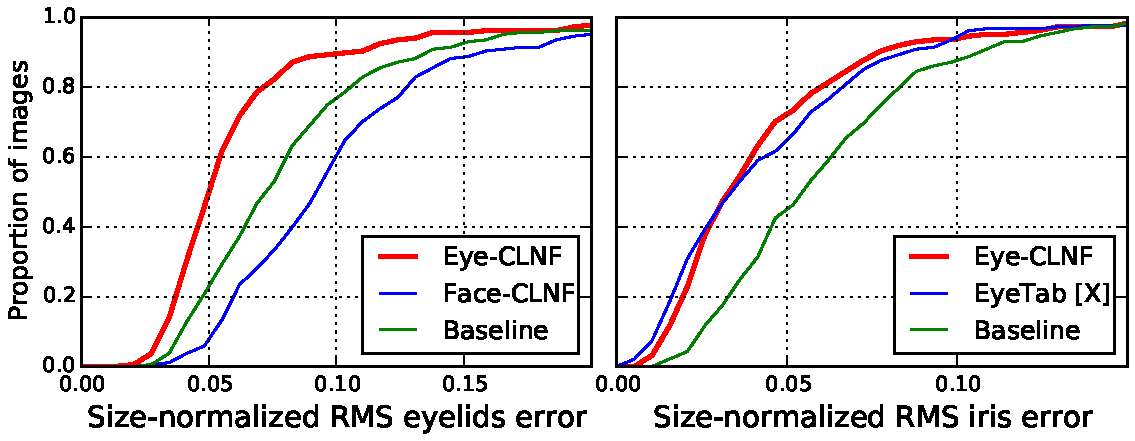
\includegraphics[width=\columnwidth]{CLNF_MPII_experiment}
    \caption{Results of annotated MPII experiment}
    \label{fig:clnf_results}
\end{figure}

\begin{figure}
    \centering
    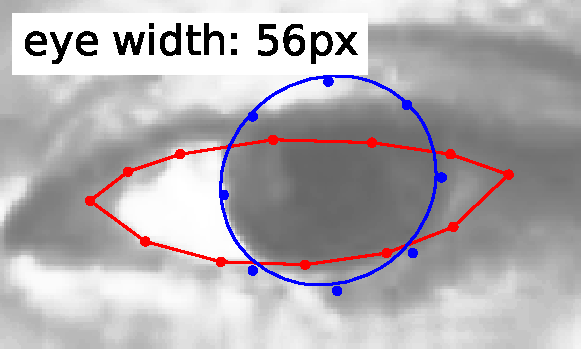
\includegraphics[width=0.244\columnwidth]{figs/ldmks_examples/idx_7.pdf}\hfill
    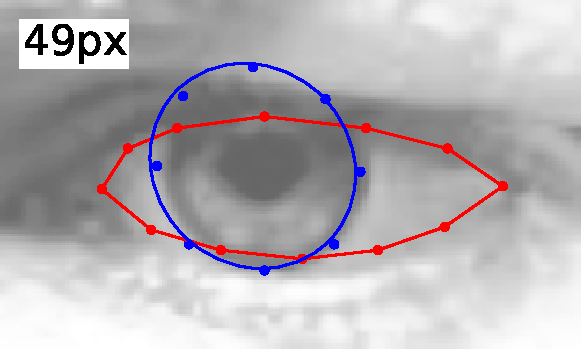
\includegraphics[width=0.244\columnwidth]{figs/ldmks_examples/idx_32.pdf}\hfill
    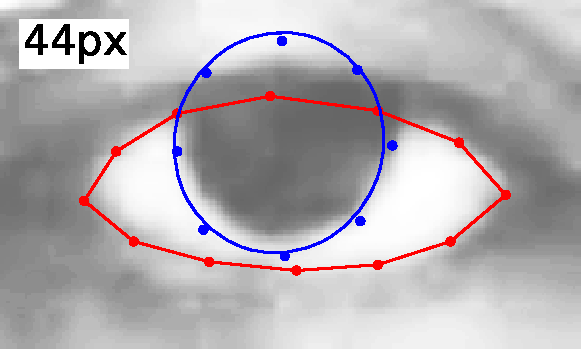
\includegraphics[width=0.244\columnwidth]{figs/ldmks_examples/idx_19.pdf}\hfill
    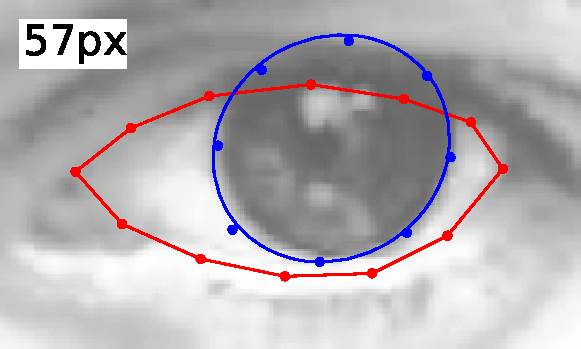
\includegraphics[width=0.244\columnwidth]{figs/ldmks_examples/idx_92.pdf}
    \par \vspace{0.1em}
    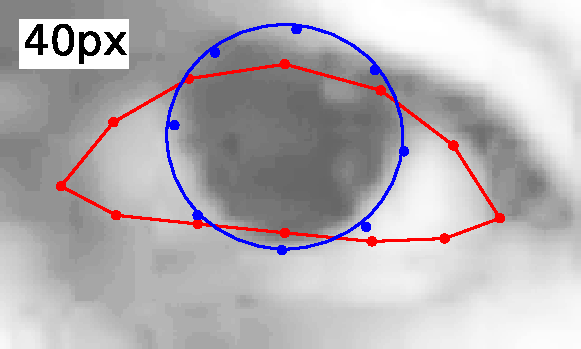
\includegraphics[width=0.244\columnwidth]{figs/ldmks_examples/idx_14.pdf}\hfill
    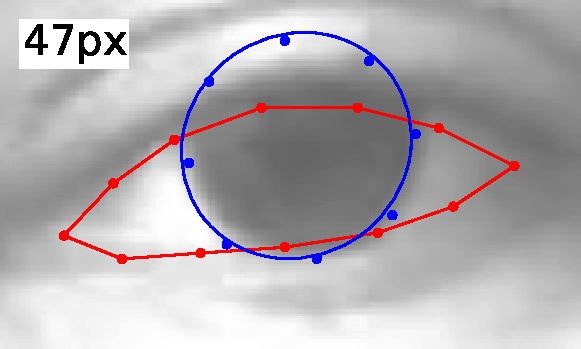
\includegraphics[width=0.244\columnwidth]{figs/ldmks_examples/idx_24.pdf}\hfill
    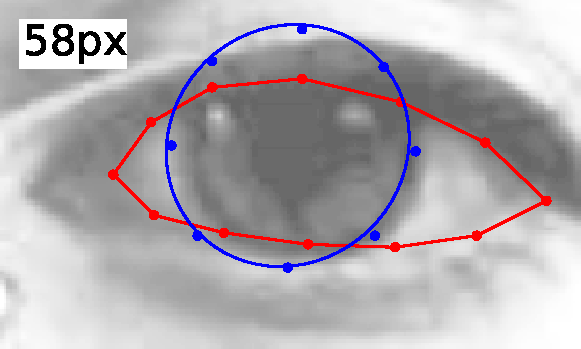
\includegraphics[width=0.244\columnwidth]{figs/ldmks_examples/idx_45.pdf}\hfill
    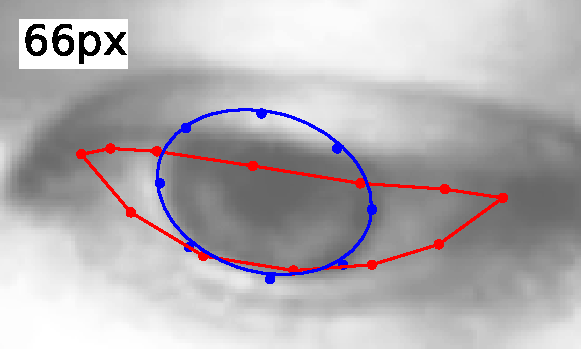
\includegraphics[width=0.244\columnwidth]{figs/ldmks_examples/idx_75.pdf}
    \par \vspace{0.1em}
    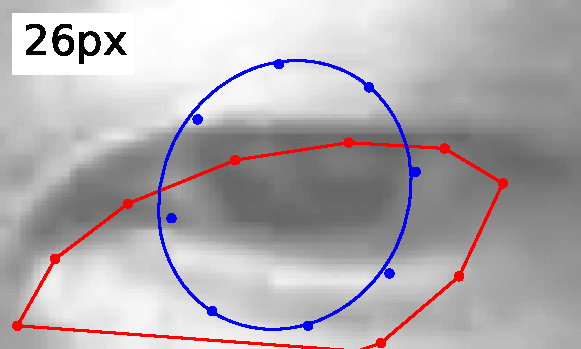
\includegraphics[width=0.244\columnwidth]{figs/ldmks_examples/idx_4.pdf}\hfill
    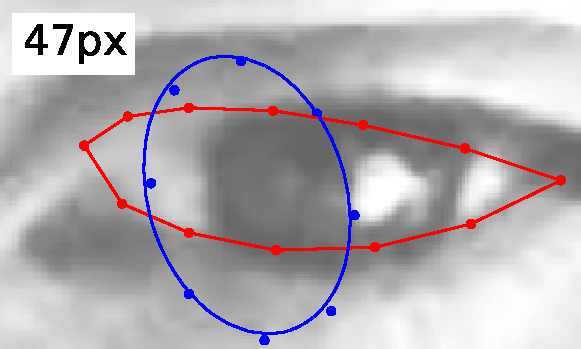
\includegraphics[width=0.244\columnwidth]{figs/ldmks_examples/idx_26.pdf}\hfill
    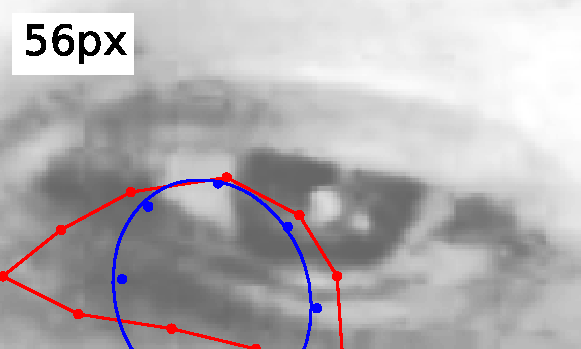
\includegraphics[width=0.244\columnwidth]{figs/ldmks_examples/idx_134.pdf}\hfill
    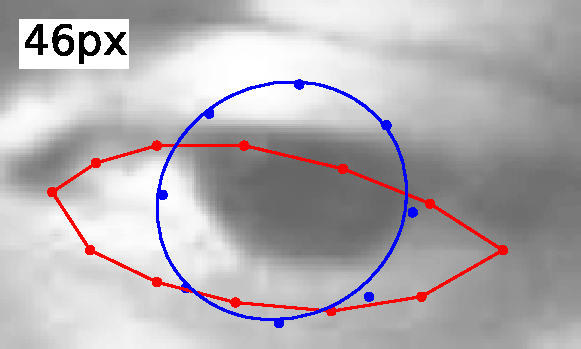
\includegraphics[width=0.244\columnwidth]{figs/ldmks_examples/idx_83.pdf}
    %
    \caption{The top two rows illustrate successful eye-region model registration on MPIIGaze. The bottom row illustrates failure cases.}
    \label{fig:clnf_examples}
\end{figure}

While the in-the-wild images represent challenging conditions for eyelid registration, they are not representitive of typical webcam-style images and do not feature labels for the iris.
We therefore annotated sub-pixel eyelid and iris boundaries onto a subset of MPIIGaze ($n\!=\!188$), a dataset collected during natural everday laptop use over several months \cite{zhang15_cvpr}.
Pupil accuracy was not evaluated as we found it was impossible to discern in in most images.
We compared our eye-region CLNF with EyeTab \cite{wood2014eyetab}, a state-of-the-art shape-based approach that robustly fits ellipses to the limbus using image-aware RANSAC \cite{swirski2012robust}.
We used the author's implementation, with their suggested modifications to improve performance: improved eyelid localization with a state-of-the-art facial landmark detector \cite{baltrusaitis2013constrained}.
As a baseline, we used the mean position of all eye-region landmarks following model initialization.
Eyelid errors were calculated as RMS distances from the eye corner and eyelid landmarks to ground truth eyelid boudnary.
Iris errors were calculated by first least-squares fitting an ellipse to the tracked iris landmarks, discretizing it at a high resolution, removing points outside ground truth and tracked eyelid boundaries, and then calculating RMS distances to the ground truth iris ellipse.
This avoided calculating errors for parts of the iris which were occluded by the eyelid.
Errors were normalized by the eye-width, and are reported using average eye-width ($44.4\!\pm\!8.85\textrm{px}$) as reference.

As shown in \autoref{fig:clnf_results}, our approach ($1.89\!\pm\!1.52\textrm{px}$) demonstrates comparable iris-fitting accuracy with EyeTab ($1.79\!\pm\!1.22\textrm{px}$), a state-of-the-art specialist algorithm for fitting ellipses to irises. However, our eye-CLM is more robust, with EyeTab failing to terminate in $2\%$ of test cases. As shown by \todo{prev exp.}, our eye-CLM ($2.79\!\pm\!2.20\textrm{px}$) also localizes eyelids better than previous state-of-the-art facial landmark trackers ($4.27\!\pm\!1.84\textrm{px}$).

% show that we only need data from few(er) people and show competitive performance
% Maybe) Plot landmark accuracy on LFW against number of training participants. Show that even with just a few participants (e.g. 4) we get good results for eyelid positions compared to state-of-the-art face trackers.

% eye corner detection
% eye bounding box detection
% eye position detection?
% ^ I think all of these come with what the deformable model gives us

\subsection{Gaze Estimation}

% evaluate eye/gaze/eyelid shapes (fully synthetic) separately from full face appearance (which is a mixture of real and synthetic data)

% person-adaptation, use pre-trained model from synthesised data, then personalise with small amount of user-specific data
% ^ let's leave this as future work! Can put it in the discussion 

% show that we can synthesise specific datasets for specific settings (specific head and gaze ranges, illumination conditions), show that we can competitive performance
We render a targeted dataset that matches MPII's gaze and pose distribution, with added 3D laptop screen emitting light. This shows how we can target specific scenarios like laptop-based gaze estimation, and render a suitable dataset within a day rather than take 3 months of data collection.

% train on synthesised images and show competitive performance on MPIIgaze with real images
% show better performance than UT dataset
Using Xucong's CNN sytem, we train on targeted version of \dataset, test on MPII. Show results are better than training on UT and testing on MPII. This shows that the range of lighting in \dataset is important for better results.

% does photorealistic data really help/is it necessary? either reduce quality and see how it affects performance, or compare model with and without shape variations
% ^ I am not really sure how to do this well... Because we'd also have to have a measure of "how photorealistic" something is. Swapping the eyeball for a simpler model, e.g. sphere might not really have that much of an effect on "photorealism" for many eye-poses. Changing the shaders, e.g. pretending the skin is Lambertian (diffuse) might?

